\DontNumberThisInToc
\DontFrameThisInToc
\ChapterNoNumberCitation{Les Ganglions de la base}{Yes I can}{}{10cm}
\section{Introduction}
\ChapterNoNumberCitation{Les Ganglions de la base}{Yes I can}{}{10cm}
 \section{Introduction}
 
-Les noyaux gris centraux appelés encore les ganglions de la base (BG, \textit{basal ganglia}) sont un ensemble de noyaux sous-corticaux interconnectés qui ont longtemps fait l'objet d'études neuroatomiques. Leur intérêt particulier est le fait que de nombreux troubles du mouvement (la maladie de Parkinson \citep{Ehringer:1960}, la maladie de Huntington \citep{Reiner:1988, Sapp:1995}, le syndrome de Tourette, etc.) chez l'homme sont dus à des maladies affectant les BG. En effet, de nombreuses études suggèrent que les BG participent à la régulation de l'activité du corticale, par désinhibition du thalamus considéré comme relais, ce qui leur permet d'avoir un rôle prémordial dans la sélection de mouvements et l'apprentissage par renforcement en assurant un ensemble d'intégrations dans des canaux distincts fonctionnellement. 
 
-%Ces ganglions, ou amas de cellules nerveuses, sont étroitement interconnectés et reçoivent également des informations en provenance de plusieurs régions du cortex cérébral. Une fois traitée par les ganglions de la base, cette information retourne au cortex moteur en passant par le thalamus.%
 
-L'entrée corticale vers BG est organisée en bandes longitudinales de projections. On distingue cinq circuits : un circuit moteur qui inclut les aires sensorimotrices précentrales, un circuit oculomoteur passant par le cortex frontal et les oculomoteurs frontaux (FEF\footnote{ C'est une zone corticale qui joue un rôle important dans le contrôle de l'attention visuelle et les mouvements oculaires. Leur stimulation électrique suscite des saccades oculaires. Ils ont une structure topographique et représentent les cibles visuelles dans les coordonnées rétinotopiques}, \textit{frontal eye field}), deux circuits préfrontaux passant respectivement par le cortex dorsolatéral préfrontal et orbitofrontal latéral et finalement un circuit limbique reliant le cortex cingulaire et orbitofrontal mdial. \citep{Alexander et crutcher 1990} Ces boucles permettes de sélectionner des états corticaux, de les intégrer et de contrôler leur succession..\citep{Berns and Sejnowski 1996,1998, Beiser and houk 1998, NAKAHARA Doya and Hikosaka 1999, 2001}
-%
-Boucles BG: Une avancée majeure dans la compréhension de la circuiterie des ganglions de la base a été la reconnaissance que ses neurones ont été organisées dans une série de boucles parallèles. Chaque boucle a commencé dans le cortex avec une excitation du striatum suivie par l'entrée de la GPi, qui a ensuite variablement inhibé le thalamus dont les projections d'excitation envoyé à nouveau sur la source d'origine corticale. Bien que cette architecture continue à être étudié, plus de cinq boucles distinctes et plusieurs connexions divergentes ont été identifiés. La boucle motorice a été le plus étudié et est mieux comprise. Cette forme d'organisation est particulièrement adapté pour des effets de rétroaction ou de feed-forward, tandis que Les interférences entre les boucles peuvent être cruciales pour les activités corrélées dans les différentes régions corticales.%
-
 \section {Anatomie}
-%%% Les ganglions de la base sont, comme leur nom l'indique, formés d'un ensemble de structures nerveuses enfouies profondément sous le cortex.%%%
 
-Plusieurs études ont été consacrées à la structure et à la physiologie des ganglions de la base \citep{Houk,Davis and Beiser 1995, Graybiel:1998, DeLong:2000}
-Les ganglions de la base peuvent être présentés comme deux structures d'entrée, deux structures de sortie et deux structures intrinsèques intermédiaires.
-Les structures d'entrées sont le striatum qui reçoit des signaux excitateurs de presque toutes les aires du cortex cérébral (sauf les aires primaires visuelle et auditive) 
-\citep{Cherubini:1988,Kemp:1970,kitai:1976,McGeer:1977} et le noyau sous-thalamique qui reçoit principalement des aires motrices du lobe frontal \citep{Fujimoto:1993, Monakow:1978, Rouzaire:1987}.
- 
-\begin{figure}[htb]
-  \begin{center}
-    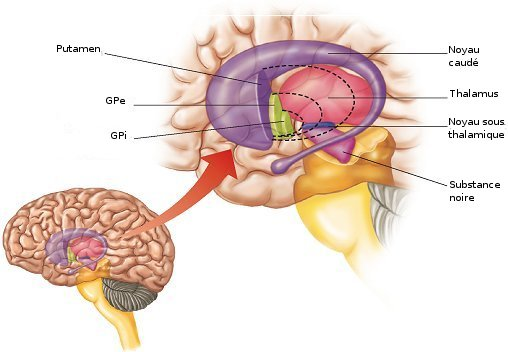
\includegraphics[width=0.6\textwidth]{Pics/BG1}
-  \end{center}
-  \caption {Les différents noyaux des ganglions de la base. Le striatum (STR) composé du noyau caudé et du putamen. Le pallidum composé du segment interne (GPi) et segment externe (GPE). La substance noire composée de la partie compacte (SNc) et la partie réticulée (SNr). Le noyau sous thalamique (STN).}
-  \label{fig:BG1}
-\end{figure}
 
-\subsection{Le striatum}
 
-Le striatum (STR, \textit{striatum}) est le plus large des noyaux gris centraux (10000000 neurones chacun connecté à 10000 synapses corticales). Il est composé du noyau caudé, du putamen et d'une partie différenciée connue sous le terme "striatum ventral"\footnote{Le striatum ventral est particulièrement impliqué dans la régulation des comportements motivés comme les processus naturels liés à l’obtention d’une récompense ou les processus pathologiques de l’addiction. %(Ikemoto and Panksepp, 1996; Koob, 1992; Koob and Bloom, 1988; Robbins et al., 1989; Robledo and Koob, 1993; Robledo et al., 1992; Salamone, 1994
-} qui englobe le noyau accumbens septi (NAcc, \textit{accumbens septi nucleus}), les parties ventromédiales du noyau caudé et du putamen et les cellules striatales des tubercules olfactifs.
-
-STR reçoit en effet de multiples afférences excitatrices glutamatergiques qui proviennent globalement de toutes les aires du cortex cérébral sauf l'aire visuelle primaire (V1, \textit{primary visual area}) et l'aire auditive primaire(A1, \textit{primary auditory area}) \citep{Albin:1995, Gerfen:1990, Cherubini:1988, Kemp:1970}. Outre le cortex, il reçoit des projections excitatrices des structures sous-corticales: thalamus (TH, \textit{thalamus}), hippocampe et amygdale \citep{Lapper:1992, Sadikot:1992}. 
-
-Il est constitué principalement ($90-90\%$) de neurones GABAergiques\footnote{L'acide $\gamma$-aminobutyrique, abrégé en GABA, est le principal neurotransmetteur inhibiteur du système nerveux central chez les mammifères et les oiseaux.} épineux moyens ( MSN, \textit{medium spiny neurons}). Au repos, ces neurones ont peu d'activité spontanée. Ils sont maintenus dans un état de faible excitabilité et sont peu réactifs aux influx corticaux excitateurs \citep{Nisenbaum:1995}. En conséquence, une forte activité synchronisée des projections cortico-striatales est nécessaire pour que les neurones de projection du striatum dépassent le seuil d'activation \citep {Mahon:2001, Mahon:2003}.
-
-Ces neurones projettent d'une part sur le segment interne du pallidum (GPi, \textit{internal globus pallidus}) et la substance noire réticulée (SNr, \textit { Substantia nigra pars reticulata}). D'autre part, ils projettent sur le noyau sous-thalamique (STN, \textit{subthalamic nucleus}) à travers le segment externe du pallidum (GPe, \textit{} external globus pallidus). Les neurones qui projettent vers un noyau ou un autre sont morphologiquement indifférenciables et topographiquement mélangés \citep{Feger:1984, Gerfen:1988, Parent:1989}. Ils commencent à décharger avant que le mouvement ne commence. Ceci suggère que le striatum participe à la programmation du mouvement en devenir. \citep{Lidsky:1985} ont signalé une activité neuronale striatale qui semblait
-être liée uniquement à des mouvements ou des stimuli sensoriels qui se produisent dans un contexte particulier. En effet, STR participe à filtrer les informations corticales les plus pertinentes et transformer les signaux corticaux selon le contexte afin d'inhiber localement les noyaux de sorties des BG permettant ainsi d'enlever l'inhibition tonique des générateurs de patterns moteurs (GPM, \textit{motor pattern generator}) reliés aux mouvements désirés mais il est également impliqué dans l'apprentissage de compétences motrices, perceptives et cognitives\citep{Joel:1994, Suzuki:2001}. 
- 
-
-\subsection{Le noyau sous-thalamique}
-
-Le noyau sous-thalamique est le seul noyau excitateur des BG, il re\c coit des projections inhibitrices du GPe et ses neurones glutaminergiques renvoient des projections
-excitatrices répandues\footnote{efférences divergentes: chaque axone de STN innerve de nombreux neurones de GPi} aux GPi et SNr \citep{Parent:1993} permettant ainsi d'inhiber les MPG des mouvements concurrents. Il reçoit principalement des afférences excitatrices des aires motrices du lobe frontal.
-
-\subsection{Le pallidum externe}
-
-Le segment externe du pallidum est une structure intermédiaire qui reçoit des projections inhibitrices de STR et d'autres excitatrices de STN et renvoie des projections GABAergiques inhibitrices vers STR et GPi mais majoritairement vers STN \citep{Rouzaire:1980}. Il semble agir en opposition aux projections striatales \citep{Alexander:1990}.
- 
-
-
-\subsection{Le pallidum interne et la substance noire réticulée}
-
-Ces deux noyaux composés de neurones similaires sont considérés comme une seule structure fonctionnelle de sortie \citep {Carpenter:1981}. Ils sont toniquement actifs, i.e déchargent au repos à des taux élevés en l'absence de l'entrée striatale leur imposant une pause ou de réduire leur cadence de décharge. Ces structures pallidaux fonctionnent en utilisant un principe de désinhibition. Ayant feu . Parce un effet inhibiteur sur leurs cibles, l'effet net de l'entrée du striatum au GPi/SNr est une réduction de l'inhibition tonique exercée par les cellules pallidiales sur leurs cibles (désinhibition) permettant donc une augmentation du taux de décharge dans les cibles (thalamus, colliculus supérieur...). Donc leur désinhibition permet en particulier d'activer les aires motrices via le thalamus par excitations glutamatergique des aires corticales frontales et d'initier ainsi les mouvements moteurs bloqués toniquement \citep{Nauta:1966}. 
-
-\section{Les inter-connexions entre les noyaux grix centraux: vue d'ensemble }
-
-
-Un schéma synthétique des circuits impliquant les ganglions de la base est présenté dans la figure \ref{BG2}. Une grande partie de l'entrée des BG arrive au niveau de striatum qui projette vers la sortie GPi/SNr via deux chemins : la "voie directe" et la "voie indirecte", qui semblent avoir des effets contraires \citep{Albin:1989}. En effet au repos, le thalamus est inhibé par GPi/SNr. L'inhibition de certains neurones peut être enlevée sélectivement via la voie directe: le striatum qui inhibe certaines neurones de GPi/SNr. La boucle qui relie le néocortex, le striatum, le palladium interne, le thalamus et le cortex frontal est classiquement considérée comme la "boucle principale" des ganglions de la base. Mais il s'y ajoute la projections en avale de la substance noire réticulée principalement vers le colliculus supérieur, participant ainsi au contrôle oculomoteur des saccades visuelles \citep{Graybiel:1978, Hikosaka:1983a, Hikosaka:1983b, Hikosaka:1983c}
-
-A cette boucle principale, s'ajoute des boucles latérales qui participent particulièrement à la régulation de l'activité de palladium comme la voie indirecte. Une fois stimulée par le cortex, les neurones du striatum dans les axones de la voie indirecte, envoient des projections inhibitrices sur les cellules du pallidum externe, qui inhibe de manière tonique le noyau sous-thalamique. Cette inhibition (par STR) des projections inhibitrices du GPE, se traduit par une réduction nette de l'inhibition de STN. Finalement STN, à son tour, envoie des projections excitatrices au complexe SNr/GPi (qui inhibe toniquement le thalamus). Le résultat final est en particulier une inhibition du thalamus et, par conséquent, une diminution de la stimulation du cortex moteur par le thalamus et l'activité musculaire est réduite.
-
-En considérant en plus l'entrée corticale vers le noyau sous-thalamique, à ces deux voies s'ajoute la "voie hyperdirecte" \citep{Nambu:2002, Joel:1997}. Une stimulation corticale induit une excitation à courte latence, suivie par une inhibition puis une excitation retardée dans les neurones pallidaux de singes. L'excitation précoce est considéré comme provenant de la voie cortico-STN-pallidale fondée sur les constatations dans \citep{Nambu:2000}. Cette voie s'avère être une voie excitatrice rapide par opposition à celles qui passent par le striatum et qui semblent être plus lentes. Le modèle de Nambu qui introduit cette voie propose de considérer que lorsque un mouvement volontaire est présenté au niveau cortical, un premier message via la voie "hyperdirecte" qui excite de manière diffuse SNr/GPi et par conséquent inhibe le thalamus et ses projections corticales. Cette inhibition affecterait non seulement les mouvements "concurrents" mais aussi le mouvement choisi (un signal de réinitialisation,\textit{"RESET"}).
-
-Il en résulte deux types de sélections par compétition entre les voies \citep{Hikosaka:1993}. D'une part, une compétition simultanée: une inhibition globale via les voies indirecte et hyperdirecte contre une désinhibition sélective via la voie directe. D'autre part, une compétition séquentielle due aux différences entre les constantes temporelles des différentes projections.
-
-\begin{figure}
-\begin{center}
-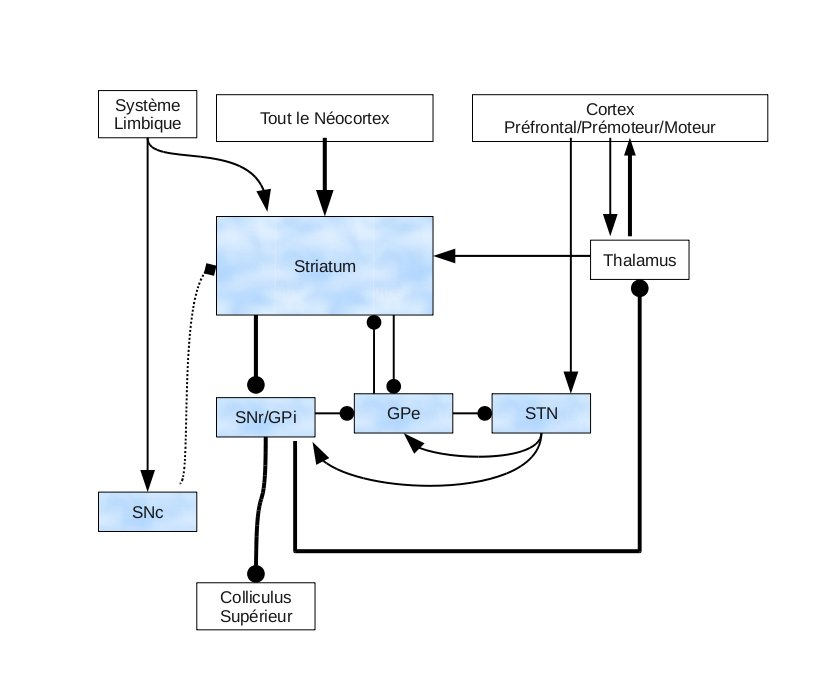
\includegraphics[width=\textwidth]{Pics/BG2}
-\end{center}
-\caption{Schéma synthétique des ganglions de la base et des principales connexions associées. Les connexions excitatrices (glutamergiques) sont représentées par des flèches en pointes rondes, les connexions inhibitrices (GABAergiques) par des flèches pleines et les connexions dopaminergiques par des flèches en pointillés. La boucle principale Cortex-BG-Thalamus-Cortex est en gras(Adapté de \citep{Graybiel:1993}).}
-\label{BG2}
-\end{figure}
-
-
-\section {Dopamine et apprentissage par renforcement dans les BG}
-
-%Voie nigrostriatale: cette projection de la dopamine est le plus dégénéré dans la maladie de Parkinson et a des projections abondantes dans le striatum, tandis que d'autres systèmes dopaminergiques ils projettent largement du cortex à la moelle épinière. Son effet de base est d'augmenter la production des noyaux gris centraux, en agissant sur les récepteurs dopaminergiques D1 dans les neurones du striatum qui stimulent la voie directe et sur les récepteurs dopaminergiques D2 qui stimulent la voie indirecte. Une grande partie de l'activité SNc tend à être tonique ou phasique soutenue plutôt que transitoire ou, ce qui a conduit à une certaine difficulté à établir la contribution explicite la voie à de commande du moteur.%
-
-
-La dopamine (DA,\textit{Dopamine})est un neuromodulateur qui est produit dans les neurones de SNc. Ces neurones projettent sur les MSN.  Le rôle de la dopamine au sein des BG est complexe et en grande partie non résolu. Globalement, la dopamine est impliquée dans deux
-fonctions fondamentales du cerveau: Activation motrice et apprentissage par récompense des associations stimulus-réponse(S-R) \footnote{choisir une action en réponse à un contexte sensoriel donné.}.
-
-En effet, les neurones de SNc peuvent agir, grâce à la dopamine, sur la réponse des neurones striataux aux entrées corticales. Les profils d'activités striatales qui peuvent être corrélées avec l'exécution de tâches suivie par une récompense sont renforcés.  
-Avec l'action de la dopamine sur les neurones du striatum, les neurones SNC peut modifier la réponse des neurones du striatum à l'entrée corticale de telle sorte que les modèles d'activité striatale qui se corrèlent avec l'exécution des tâches résultant de récompense sont renforcés par l'augmentation de la force (poids) synaptique des entrées corticales.
-
-
-La dopamine a d'abord été considérée comme un signal de récompense. Plusieurs enregistrements électrophysiologiques, chez des singes apprenant des tâches comportementales, ont montré des neurones dopaminergiques qui déchargent de façon phasique quand une récompense inattendue arrive mais quand la même expérience est répétée plusieurs fois, la décharge se décale dans le temps pour répondre aux stimulus prédisant ainsi la récompense et ne plus coïncider donc avec à la récompense. La dopamine est ainsi considérée comme un signal d'erreur de récompense (corrélée donc avec l'anticipation de la récompense) et non plus un signal de récompense\citep{Houk:1995, Schultz:1997, Hollerman:1998}.
-%L'analogie entre les noyaux gris centraux et acteur-modèles de porte-parole s'appuie sur la forte ressemblance entre les DA activité du neurone et le signal d'erreur de prédiction TD, et entre DA-dépendante à long terme la plasticité synaptique dans le striatum (Calabresi et al, 2000;. Wickens, Begg, et Arbuthnott, 1996) et de l'apprentissage guidé par une prédictionsignal d'erreur en l'acteur.
-
-\section{Théories sur les fonctions des BG}
-
-%Les systèmes corticaux sont assez bien connus, et sont à l’origine du plan moteur. En revanche, les ganglions de la base restent moins bien explorés : ils sont à l’origine de la maturation du projet moteur, et permettent sa réalisation effective. Leur étude est très importante, car il sont impliqués dans plusieurs pathologies importantes. Ces ganglions sont également impliqués dans des fonctions plus cognitives, comme le traitement des émotions, de la mémoire, des comportements. D’autres voies nerveuses sont alors mis en œuvre. %
-Alors que les fonctions des ganglions de la base font office de médiateur non motrices de nombreux y compris la cognition, l'émotion et le traitement sensoriel, ils ont longtemps été considérées comme étant principalement impliqué dans le mouvement.
-
-%--------------------------------------------------------------------
-\subsection{Réduire la dimensionnalité de l'information corticale}
-
-L'idée est de considérer les BG comme un commutateur adaptatif central qui ordonne les informations entrantes selon les priorités et les compresse pour activer le cortex frontal à travers un nombre limité de canaux. Deux stratégies sont proposés, réduire la dimensionnalité (PCA,\textit{Principal Component Analysis}\footnote{}) ou bien réduire l'information (Clustering\footnote{}).\citep{Bar-gad extraction methods}
-
-BG servent  à réduire la dimensionnalité de l'information corticale à l'aide des méthodes d'extraction optimales
-
-%--------------------------------------------------------------------
-
-\subsection{Séléctionner une commande et supprimer le reste}
-Pour générer a movement, il n'est pas suffisant d'activer le MPG souhaité  à cause de la présence de MPG concurrents qui sont préalablement activé et doivent se désactiver.
-\citep{C.Oreilly J.Frank}
-
-
-%--------------------------------------------------------------------
-
-\subsection{Sélection de l'action}
-BG forment un mécanisme de sélection qui décide des compétitions entre les actions alternatives disponibles dans un contexte donné.
-\citep{Gurney,redgrave,Mchaffie}
-
-%--------------------------------------------------------------------
-
-\subsection{Apprentissage par renforcement}
-
-\citep{Doya 1999}La dopamine code pour le prediction de la récompense $DA(t)=r(t)+1/[(V(t+1)-V(t)]$ \citep{Schultz 1997}.
-1-reactive action selection :most premitive adaptive action selection is implemented by the actor-critic architecture \citep{Barto, anderson 1983}
-2-predective action selection:conjunction with environmental dynamics Bellman equation discrete model (td error), differential model 
-3-predicion,simulation,encapsulation
-\citep{doya 2007}
-deux classes d'algorithmes : model free : model based
-reinforcement learning : 1-predict reward (value function, action value)récompense immédiate ou à long terme, 2-select action: greedy, baltzmann, 3-updateprediction:tderror
-
-La dopamine code td error\citep{Schultz:1997}
-La plasticité dépend de la dopamine \citep{wickebs:1995}
-
-Monkey free choice task \citep{Samejima 2005} representation of action specific reward values in the striatum.
-Bayesian Inference of learning process \citep{Samejima 2004}.
-learning algorithms \citep{doya 1999}.
-multiple action selection schemes\citep{doya 1994}
-
-\citep{C.Oreilly J.Frank} apprentissage pavlovien
-
-
-
-%--------------------------------------------------------------------------
-\subsection{Learning and memory functions of BG}
-
-\citep{Packard}
-stimulus-réponse association, Q learning (4paramètres : taux d'apprentissage, taux d'oubli, renforcement par récompense, aversion par absence de récompense)
-\citep{Hamker,memory retrieval in rewarded visual tasks}
-Taches visuelles de mémorisation, apprentissage par récompense-+
-
-%--------------------------------------------------------------------
-
-\subsection{planification,produire des séquences}
-
-\citep{houk 1995}analyse contextuelle de l'utilisation l'environnement et d'adaptation de l'information acquise en vue de planifier et d'exécuter des comportements intelligents 
-\citep{Berns} il a utilisé le modèle de selection de l'action de gurney en soulignant les differences temporelles possibles entre la voie directe et la voie indirecte dans un model basé seulement sur les connections intrinsèques en aval(feed-forward) des ganglions de la base.
-
-%--------------------------------------------------------------------
-
-\subsection{initiation}
-
-%L’une des fonctions de cette boucle, qui s’ajoute à celle impliquant le cervelet, est vraisemblablement de sélectionner et de déclencher des mouvements volontaires harmonieux. Ce rôle dans l'initiation et le bon déroulement de la commande motrice apparaît clairement chez les personnes dont les ganglions de la base sont endommagés, comme c’est le cas lors de la maladie de Parkinson par exemple. On observe alors chez ces patients de la difficulté à commencer les mouvements qu'ils ont planifiés, des tremblements ainsi qu’une lenteur dans l’exécution de leurs gestes.%
-
-%--------------------------------------------------------------------
-
-\subsection{BG: parallel and integrative networks}
-
-\citep {Haber} interaction entre boucles Cortex-BG 
-\citep{leblois} competition between feedback loops 
-
 



